\documentclass[conference]{IEEEtran}
\usepackage{cite}
\usepackage{hyperref}
\usepackage{graphicx}
\usepackage{amsmath,amssymb,amsfonts,bm}
\usepackage{algorithmic}
\usepackage{textcomp}
\usepackage{xcolor}
\usepackage[caption=false,justification=centering]{subfig}

\newcommand*{\vertbar}{\rule[-1ex]{0.5pt}{1.5em}}
\newcommand*{\horzbar}{\rule[0.5ex]{1.5em}{0.5pt}}

\def\BibTeX{{\rm B\kern-.05em{\sc i\kern-.025em b}\kern-.08em
    T\kern-.1667em\lower.7ex\hbox{E}\kern-.125emX}}
\begin{document}

\title{Lossy Image Compression}

\author{Reed Foster}

\maketitle

%\begin{abstract}
%Image 
%\end{abstract}
%
%\begin{IEEEkeywords}
%    Image compression, jpeg, wavelet transform, discrete cosine transform, singular value decomposition
%\end{IEEEkeywords}

\section{Introduction}

Image compression is an important area of study due to the ever-increasing consumption of media and explosion of big data image processing \cite{imgProcessingTinkuAcharya}, \cite{scnn}.
The goal of lossy image compression is to preserve the perceptually relevant portions of an image so that the image appears unaltered while drastically reducing the number of bits required to store the image.

In this paper, I will discuss several methods of image compression and evaluate their performance on metrics of image quality and compression ratio.

\section{Background}

\subsection{Perception}
Images are often represented as 3 separate channels of the red, green, and blue intensity at each pixel in the image.
However, because humans are more sensitive to some colors but not others, and are more sensitive to different hues when they are of different brightnesses or intensities, this is not the best way to encode images for compression.
JPEG uses the $YC_bC_r$ image representation, where $Y$ is the luma or brightness component and $C_b$ and $C_r$ are the blue and red difference components (i.e. $C_b = B - Y$, $C_r = R - Y$).
The human eye is most sensitive to the information in the $Y$ channel, but less sensitive to changes in red and blue color, so this leaves an opportunity to apply higher compression to the $C_b$ and $C_r$ channels to achieve higher compression ratios while maintaining similar image quality.

Humans perceive the different spatial frequencies in images with varying degrees of sensitivity \cite{hvsWavelet}.
State of the art lossy image compression systems (e.g. JPEG and JPEG2000 from the Joint Photographic Experts Group) leverage this to dramatically shrink the number of bits required to encode an image while maintaining a strong resemblance of the original image \cite{jpegStd}.
In order to do this, the original image is transformed into a frequency representation and the frequency representation is quantized in order to reduce the number of bits required to store it.
The quantized frequency-domain representation is then passed through lossless entropy coding to produce a compressed bitstream that can be stored or transmitted and then decoded to reconstruct the original image.
The two most popular approaches for this transformation are the discrete cosine transform (DCT) and discrete wavelet transform (DWT).

\subsection{Discrete Transforms in 1D and 2D}

A frequency transform in general can be viewed as a series of inner products between the input vector and a set of basis vectors.
Often, these basis vectors are chosen to be orthogonal (such as in the DCT and many variants of the DWT).
A one-dimensional transform of an input vector $\mathbf{x}$ can be represented as:

\begin{IEEEeqnarray}{rCl}
    \mathbf{\widetilde{x}} & = & \mathbf{\Phi}\mathbf{x} \\
    \mathbf{\Phi} & = & \begin{pmatrix}\horzbar~\bm{\varphi}^T_1~\horzbar\\\vdots\\\horzbar~\bm{\varphi}^T_N~\horzbar\end{pmatrix}
\end{IEEEeqnarray}

where $\bm{\varphi}_k$ are the basis vectors of the transform.
Each of the elements $\widetilde{x}_k$ of $\mathbf{\widetilde{x}}$ is a coefficient which measures the degree to which the input signal $\mathbf{x}$ is orthogonal to the corresponding basis vector $\bm{\varphi}_k$.
For a discrete fourier transform, these basis vectors are simply complex exponentials, with different frequencies for different basis vectors:

\begin{equation}
    \bm{\varphi}_k = \begin{pmatrix} 1, e^{-\frac{2i\pi k}{N}}, e^{-\frac{4i\pi k}{N}}, \dots e^{\frac{2(N-1)\pi k}{N}} \end{pmatrix}^T
\end{equation}

Intuitively, a discrete transform of 2D data (e.g. a matrix) can be performed by first taking a discrete transform of each individual column:
\begin{equation}
    \mathbf{\widetilde{X}}_c = \begin{pmatrix}
        \horzbar~\bm{\varphi}^T_1~\horzbar\\\vdots\\\horzbar~\bm{\varphi}^T_N~\horzbar
    \end{pmatrix}
    \begin{pmatrix}
        \vertbar && \vertbar \\
        \mathbf{x}_1 & \dots & \mathbf{x}_N \\
        \vertbar && \vertbar \\
    \end{pmatrix}
\end{equation}

Then taking a discrete transform of each row of the partially transformed matrix:
\begin{IEEEeqnarray}{rCl}
    \mathbf{\widetilde{X}}^T & = & \mathbf{\Phi}\mathbf{\widetilde{X}}^T_c \\
    \mathbf{\widetilde{X}} & = & \mathbf{\Phi}\mathbf{X}\mathbf{\Phi}^T
    \label{eqn:2Dtransform}
\end{IEEEeqnarray}

\subsection{Discrete Cosine Transform and Discrete Wavelet Transform}

For a discrete cosine transform, the basis vectors are evenly spaced in frequency.
They are given by:

\[
    \bm{\varphi}_k = \begin{pmatrix} \cos\frac{\pi k}{2N}, \cos\frac{3\pi k}{2N}, \dots \cos\frac{(2N-1)\pi k}{2N} \end{pmatrix}^T
\]

The angular frequency of the $k$th basis vector is $k\pi/N$ and the phase offset is $k\pi/2N$.

\begin{figure}[htbp]
    \centering
    \subfloat[Grayscale Image of Mandrill]{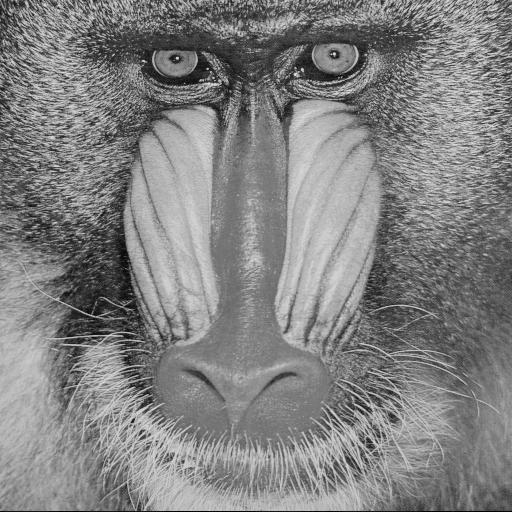
\includegraphics[width=0.8\columnwidth]{images/mandrill_gray.png}\label{fig:origGray}}
    \par\bigskip
    \subfloat[Linear Scale DWT of Image]{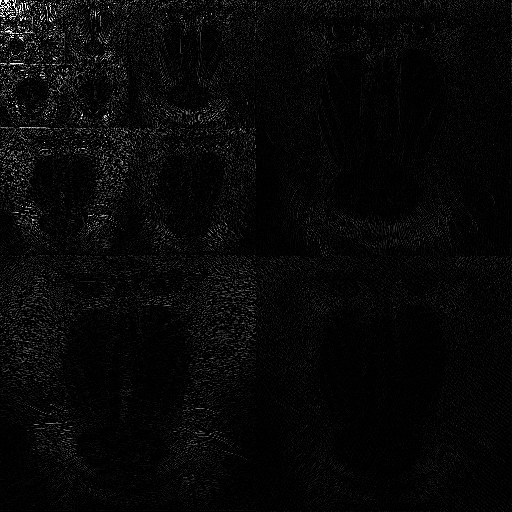
\includegraphics[width=0.8\columnwidth]{images/mandrill_linDWT.png}\label{fig:linDWTGray}}
    \par\bigskip
    \subfloat[Linear Scale DWT of Image]{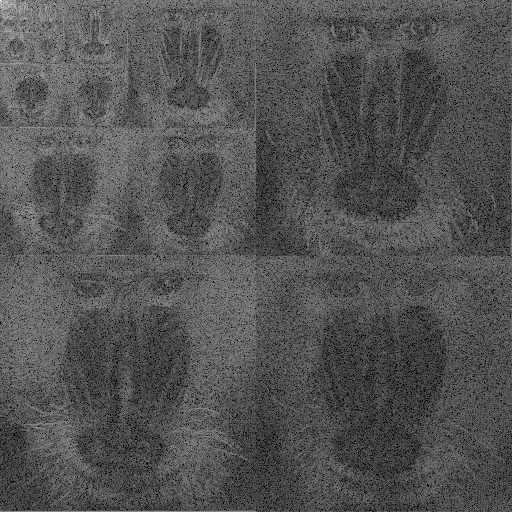
\includegraphics[width=0.8\columnwidth]{images/mandrill_logDWT.png}\label{fig:logDWTGray}}
    \caption{Discrete Wavelet Transform of an image. The Cohen-Daubechies-Feauveau 9/7 (cdf97) wavelet used in JPEG2000 was selected for this transform.}
    \label{fig:dwtImage}
\end{figure}

Unlike the discrete cosine transform, which allocates equal bandwidth for each coefficient, discrete wavelet transform basis vectors (wavelets) trade off frequency and spatial resolution.
The wavelets which have low frequency content (which will be maximally orthogonal to signals with low frequency and thus yield a large transform coefficient value) have poor spatial resolution but very fine frequency resolution.
Similarly, basis vectors with high frequency content are broadband in nature due to their temporally/spatially-localized structure.
The discrete wavelet transform is typically implemented as a set of cascaded filters and downsamplers.
The input signal is passed through a quadrature mirror filter consisting of a high pass and low pass filter.
Both filter outputs are decimated by a factor of 2, and the low pass filter output is recursively cascaded through another quadrature mirror filter pair.
This pattern of downsampling and recursively filtering the low pass output can be seen in Figure \ref{fig:logDWTGray}.
Because this is in two dimensions, each portion of the image is filtered twice: once by row and once by column.
The resulting transform domain is comprised of many ``subbands", where each subband corresponds to the output of a filter step.
The HH$_1$ subband is the portion of the image that has been high-passed both by row and by column (i.e. the bottom right quarter of the image in Figure \ref{fig:logDWTGray}).
LH$_1$ and HL$_1$ have received one high pass and one low pass each (the top right and bottom left quarters of the image in Figure \ref{fig:logDWTGray}).
Subsequent subbands received a low pass filter to both column and row, and then were downsampled and passed through another set of filters.

\subsection{Singular Value Decomposition}

A matrix can be represented as a singular value decomposition.
Singular values $\sigma_i$ of a matrix $\mathbf{A}$ satisfy

\begin{equation}
    \mathbf{A}\mathbf{v}_i = \sigma_i\mathbf{u}_i
\end{equation}

with orthonormal $\mathbf{v}_i$ and $\mathbf{u}_i$ forming an eigenbasis for $\mathbf{A}^T\mathbf{A}$ and $\mathbf{AA}^T$ (respectively).
The singular value decomposition of an $m\times n$ matrix $\mathbf{A}$ of rank $r$ can be written as so

\begin{equation}
    \mathbf{A} = 
    \begin{pmatrix}
        \vertbar && \vertbar \\
        \mathbf{u}_1 & \cdots & \mathbf{u}_m \\
        \vertbar && \vertbar \\
    \end{pmatrix}
    \begin{pmatrix}
        \sigma_1 &&&\text{\Large0} \\ 
        & \ddots && \\
        && \sigma_r & \\
        \text{\Large0}&&& 0 \\
    \end{pmatrix}
    \begin{pmatrix}\horzbar~\bm{v}^T_1~\horzbar\\\vdots\\\horzbar~\bm{v}^T_n~\horzbar\end{pmatrix}
\end{equation}

Due to Eckart and Young, we know that the rank $k$ matrix $\mathbf{A}_k$ which is constructed from the first $k$ singular values of $\mathbf{A}$ minimizes the mean square error $\left\lVert\mathbf{A}-\mathbf{A}_k\right\rVert$ \cite{strang}.

\begin{figure}[htbp]
    \centering
    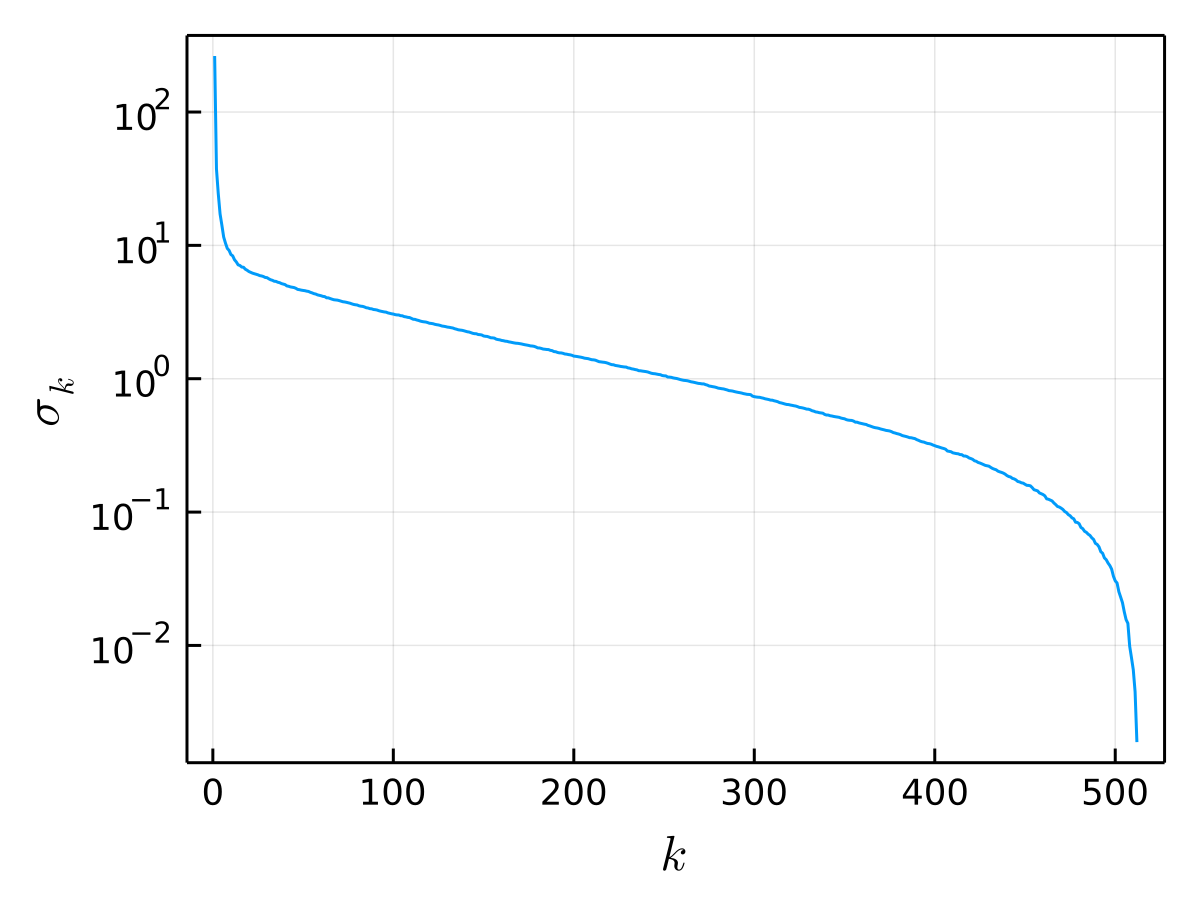
\includegraphics[width=0.7\columnwidth]{images/mandrill_SVD.png}
    \caption{Singular Values of Mandrill Image}
    \label{fig:svd}
\end{figure}


As shown in Figure \ref{fig:svd}, some singular values are very small compared to the largest singular values.
This leaves an opportunity for image compression through rank reduction.
The number of nonzero values required to store the SVD of a matrix can be calculated from the number of nonzero values in the 3 matrices of the SVD.
In $\mathbf{U}$, each basis vector $\mathbf{u}_i \in \mathbb{R}^m$ has $m$ elements.
For a rank $k$ truncation of the SVD, only $\mathbf{u}_1$ to $\mathbf{u}_k$ are needed, meaning $\mathbf{U}$ can be stored with $mk$ nonzero values.
Similarly, $nk$ nonzero values are required to store $\mathbf{V}^T$, and $k$ values to store the diagonal matrix of singular values $\bm{\Sigma}$.
Thus, the SVD can be compactly stored with $k(m + n + 1)$ nonzero values, provided $k \ll m,n$.
Storing the original $m\times n$ matrix of rank $r$ takes $mn$ nonzero values, so the rank-reduced SVD representation is not useful for compression if $k \approx m,n$.

\subsection{Lossless Compression - Entropy Coding}

The focus of this paper is not in entropy coding and lossless compression so there will be minimal discussion of these topics beyond this section.
Rank truncation and quantization reduce the number of nonzero values required to represent an image, but in order to actually store the information required to reconstruct the image, this sparsity must be leveraged by an entropy coding scheme.
JPEG (the 1992 standard) uses run length encoding and Huffman codes to create a compact representation of the quantized DCT representation of the image.
JPEG2000 uses arithmetic coding.
Because run length encoding is quite simple to understand and implement, I selected to also perform run length encoding and use the bitlength of a run-length-coded image as a compression ratio metric.
However, I will also report the sparsity of the transform-domain representation of the image (relative reduction in nonzero values in the image) as a compression ratio metric.
Even though this number-nonzero (NNZ) ratio is not a great metric for compression ratio (since having 10x fewer nonzero values doesn't guarantee that the image will require 10x fewere bits to store), it is a good indication of sparsity of values, which is extremely useful in machine learning applications, where exploiting sparsity can dramatically reduce energy consumption and improve throughput \cite{scnn}.

\section{Methods}

\subsection{Proposed Image Compression Techniques}

I implemented two DCT-based image compression techniques: one using the JPEG tiling and quantization scheme and one using an adaptive thresholding scheme.
I also implemented several DWT-based schemes.
I chose the Cohen-Daubechies-Feauveau 9/7 (cdf97) wavelet for computing the DWT because it is used in the JPEG2000 compression algorithm.
One is quite similar to JPEG2000, and uses scalar quantization.
Another uses the same adaptive thresholding scheme as in the DCT-thresholding compression technique.
Finally, I implemented a rank-truncation method which uses a reduced rank SVD representaiton of the image to reduce the number of bits required to store it.

\subsection{DCT Quantization and Thresholding}
The JPEG-like compression scheme is identical to the 1992 JPEG standard, except it doesn't implement Huffman coding to further compress the run-length encoded image, and it allows for separate quality factors (a measure of compressed image quality on a scale of 1-100) for each $YC_bC_r$ channel.

The adaptive thresholding method allows for arbitrary tile sizes (whereas the JPEG quantization method forces the tile size to 8x8).
The DCT of each $m\times m$ tile is scanned and the $n$ smallest transform coefficients are set to 0, where $n/m^2$ is the requested threshold ratio.
Larger tiles prevent ``accidental" removal of more pertinant transform coefficients, however smaller tiles can often produce a higher compression ratio.

\subsection{DWT Quantization and Thresholding}
The DWT-based quantization compression method uses scalar compression on each subband of the wavelet transform of the entire input image.
Different scalar quantization coefficients are selected for each subband, with the highest frequency subband receiving the highest level of quantization due to the fact that it typically contains very little pertinent information.
The amount of quantization (i.e. the magnitude of the quantization coefficient) is reduced exponentially for the lower frequency subbands.
The level of quantization is specified with a quality factor for each $YC_bC_r$ channel, just like the JPEG-like DCT quantization method.

The DWT adaptive thresholding method operates identically to the DCT thresholding method, except it operates on the DWT of the entire image instead of the DCT of small tiles of the image.

\subsection{SVD Compression}
Using the SVD of the original image as a technique for image compression yields quite poor results for useful compression ratios (see Figure \ref{fig:svd}; the number of negligible singular values is quite small).
Instead, the SVD of the discrete wavelet transform of the entire image is used.

\subsection{Quantifying Image Quality}

The most common metric to quantify image quality is the mean squared error of the image, which is defined for a single channel as

\begin{equation}
    MSE_{1} = \frac{1}{MN}\sum_{m,n}\left(\mathbf{X}_{m,n} - \mathbf{\hat{X}}_{m,n}\right)^2
\end{equation}

where $\mathbf{X}$ is the original $M\times N$ image and $\mathbf{\hat{X}}$ is the compressed image.
The mean squared error for the euclidean RGB distance between two colors is calculated as

\begin{equation}
    MSE_{RGB} = \frac{1}{3MN}\sum_{\mathbf{X}\in\{\mathbf{R},\mathbf{G},\mathbf{B}\}}\sum_{m,n}\left(\mathbf{X}_{m,n} - \mathbf{\hat{X}}_{m,n}\right)^2
\end{equation}

This is a pretty good metric for assessing the quality of color images.
However, the perceptual color model $\Delta E$ (CIEDE2000) from CIE, provides a better metric of image quality.
The $\Delta E$ mean squared error can be calculated as:

\begin{equation}
    MSE_{\Delta E} = \frac{1}{MN}\sum_{m,n}\Delta E\left(\mathbf{X}, \mathbf{\hat{X}}\right).^2
\end{equation}

where $\Delta E(\mathbf{X}, \mathbf{\hat{X}})$ computes the perceived difference between the 3-channel colors $\mathbf{X}$ and $\mathbf{\hat{X}}$.
This is the metric that I will use when reporting the quality of images produced by the proposed compression schemes.

Often, these mean squared error quantities are reported as a peak signal-to-noise ratio or PSNR:

\begin{equation}
    PSNR = 10\log_{10}\left(\frac{MAX_I^2}{MSE}\right)
\end{equation}

where $MAX_I$ is the maximum pixel value of the input $\mathbf{X}$ used to compute the mean squared error.

\subsection{Estimating Compression Ratio}

As mentioned in the section on entropy coding, the focus of this work is not on lossless compression techniques, so the compression ratio of these methods will be estimated with the relative increase in sparsity of the transform of the image and the number of bits required to store a run length encoding of the transform.
Explicitly, these are calculated as:
\begin{equation}
    \frac{1}{cr_{RLE}} = \frac{n_{bits}}{24RC}
\end{equation}
\begin{equation}
    \frac{1}{cr_{NNZ}} = \frac{n_{nonzero,compressed}}{n_{nonzero,orig}}
\end{equation}
where the number of nonzero values $n_{nonzero}$ counts the number of nonzero values in the transform domain.
In the case of the compression method which relies solely on SVD rank-reduction, the compression ratio is measured as the relative reduction in bits required to store the sparse SVD representation of the image's wavelet transform.

\subsection{Test Images}

A variety of test images were selected to benchmark the proposed compression algorithms; some with a lot of busy detail and others with large flat portions.
The test images are shown in Figure \ref{fig:testimages}.
\begin{figure}
    \centering
    \subfloat[mandrill]{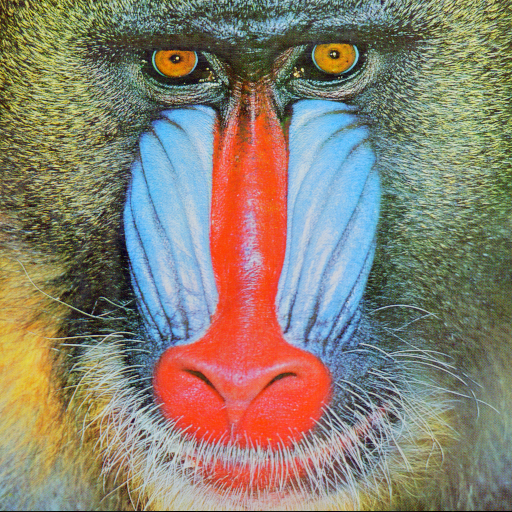
\includegraphics[width=0.3\columnwidth]{images/mandrill_orig.png}}
    \quad
    \subfloat[peppers]{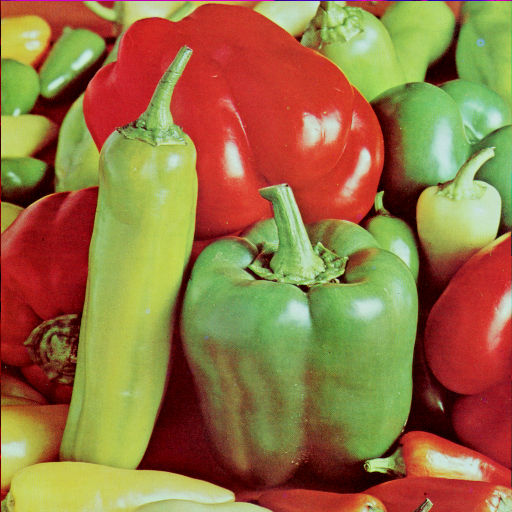
\includegraphics[width=0.3\columnwidth]{images/peppers_orig.png}}
    \quad
    \subfloat[lighthouse]{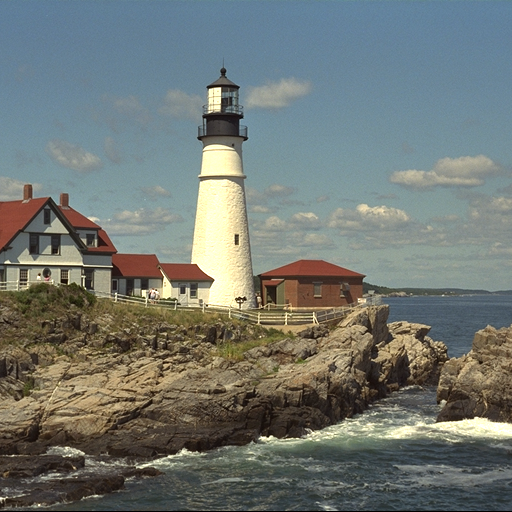
\includegraphics[width=0.3\columnwidth]{images/lighthouse_orig.png}}
    \par
    \subfloat[monarch]{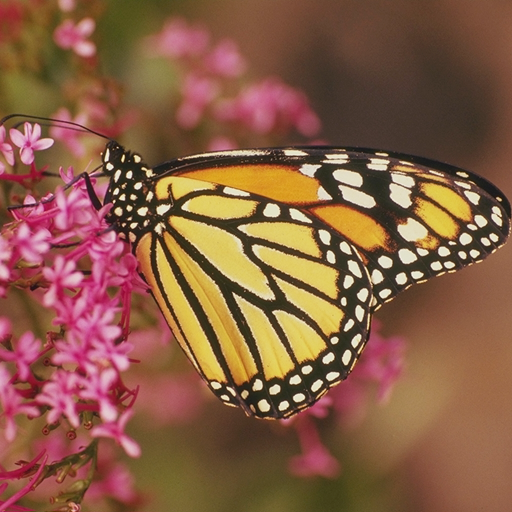
\includegraphics[width=0.3\columnwidth]{images/monarch_orig.png}}
    \quad
    \subfloat[airplane]{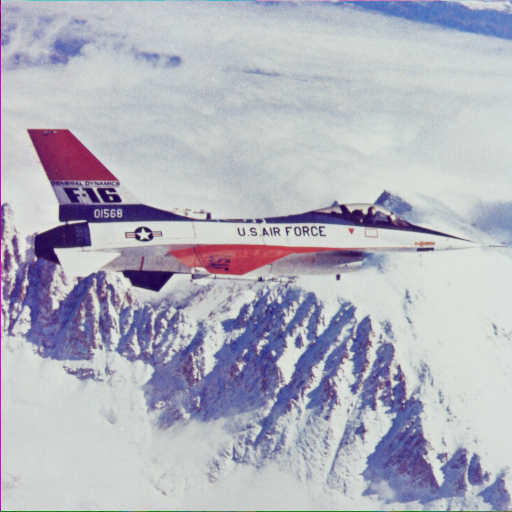
\includegraphics[width=0.3\columnwidth]{images/airplane_orig.png}}
    \caption{Test image set. All images are 3-channel RGB $512\times512$ images.}
    \label{fig:testimages}
\end{figure}

\section{Results}


\begin{figure}
    \centering
    \subfloat[mandrill (RLE)]{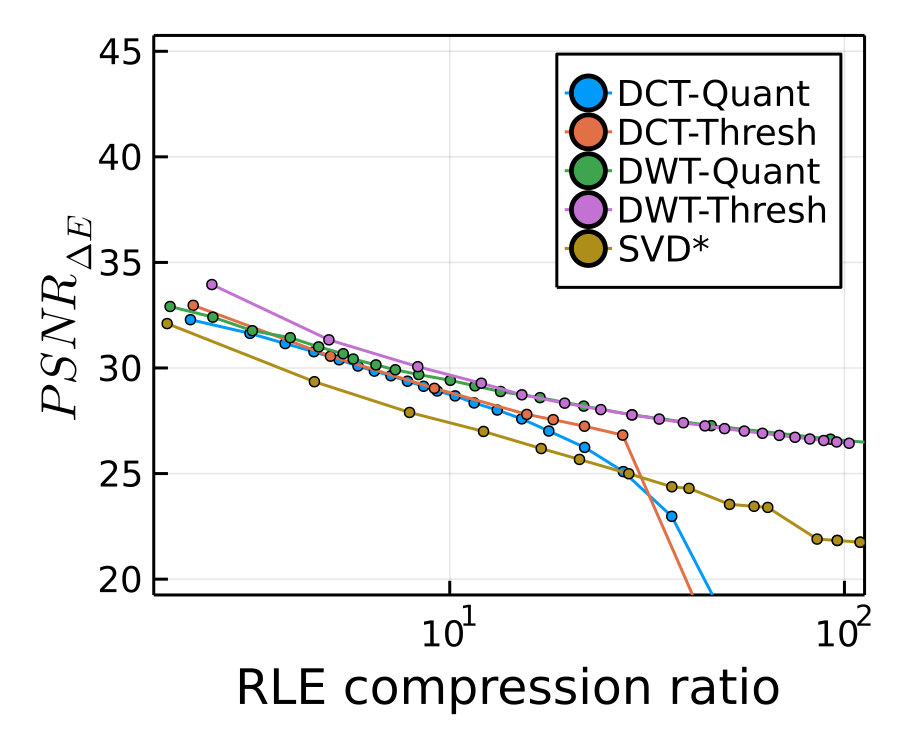
\includegraphics[width=0.48\columnwidth]{images/cr_psnr_plots/mandrill/comparison.png}}
    \quad
    \subfloat[mandrill (NNZ)]{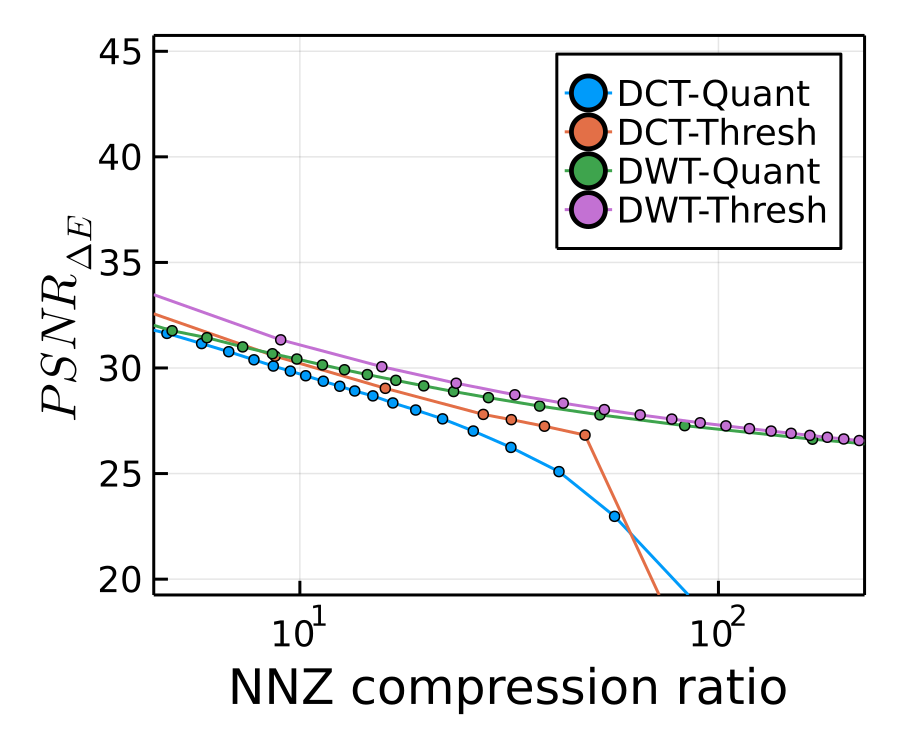
\includegraphics[width=0.48\columnwidth]{images/cr_psnr_plots/mandrill/nnz_comparison.png}}
    \par
    \subfloat[peppers (RLE)]{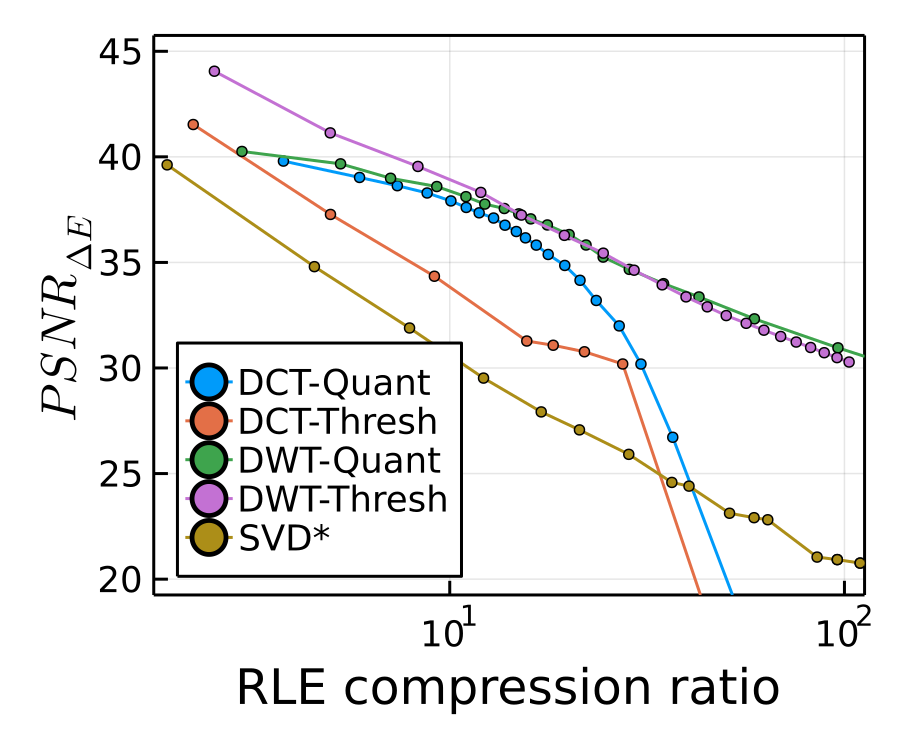
\includegraphics[width=0.48\columnwidth]{images/cr_psnr_plots/peppers/comparison.png}}
    \quad
    \subfloat[peppers (NNZ)]{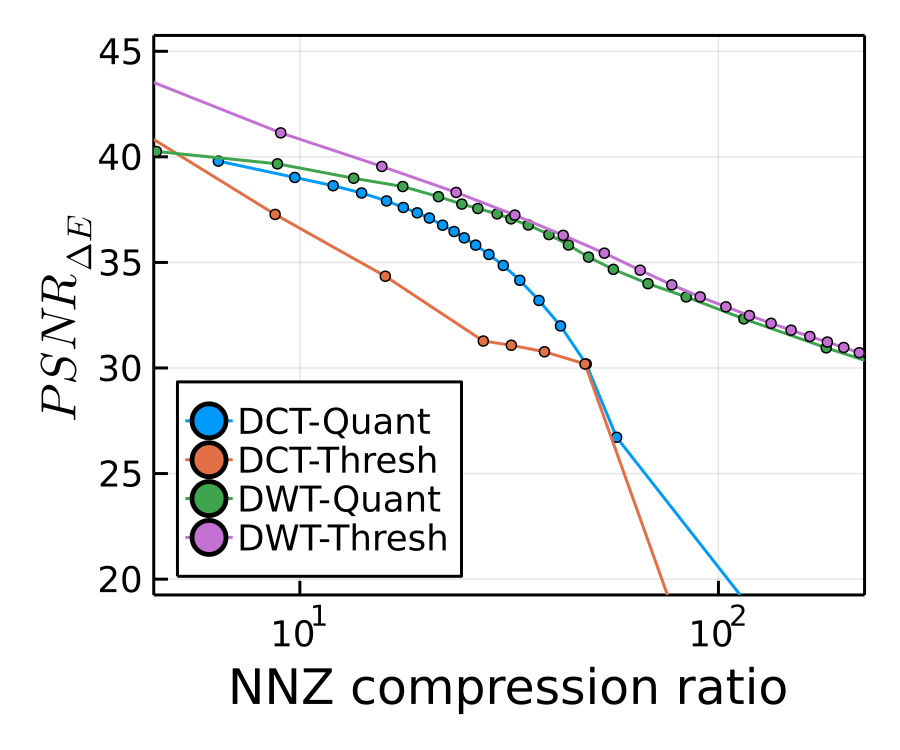
\includegraphics[width=0.48\columnwidth]{images/cr_psnr_plots/peppers/nnz_comparison.png}}
    \par
    \subfloat[lighthouse (RLE)]{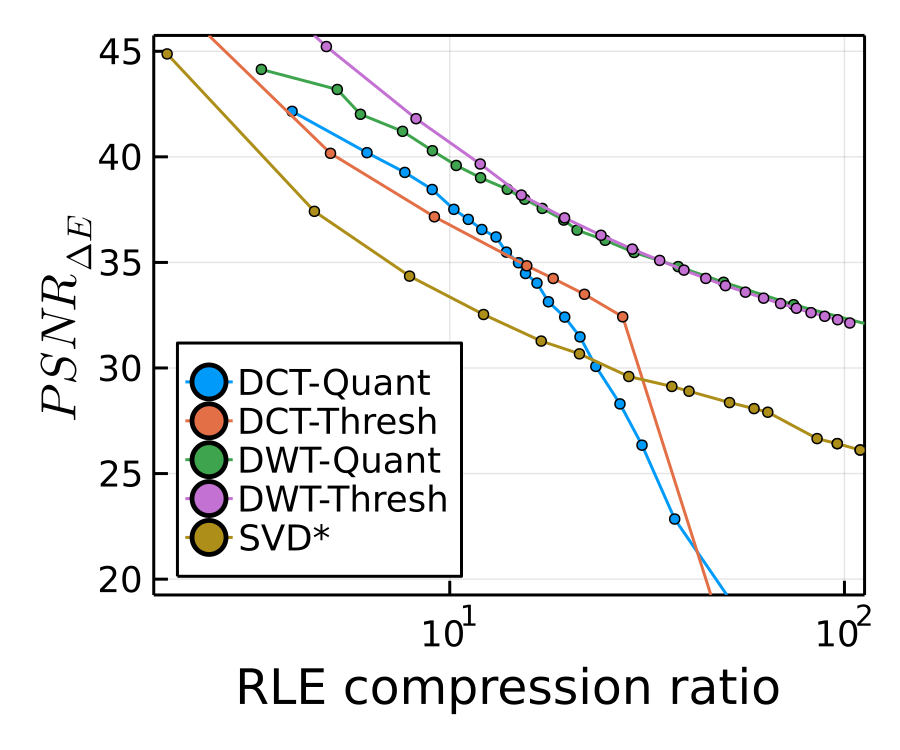
\includegraphics[width=0.48\columnwidth]{images/cr_psnr_plots/lighthouse/comparison.png}}
    \quad
    \subfloat[lighthouse (NNZ)]{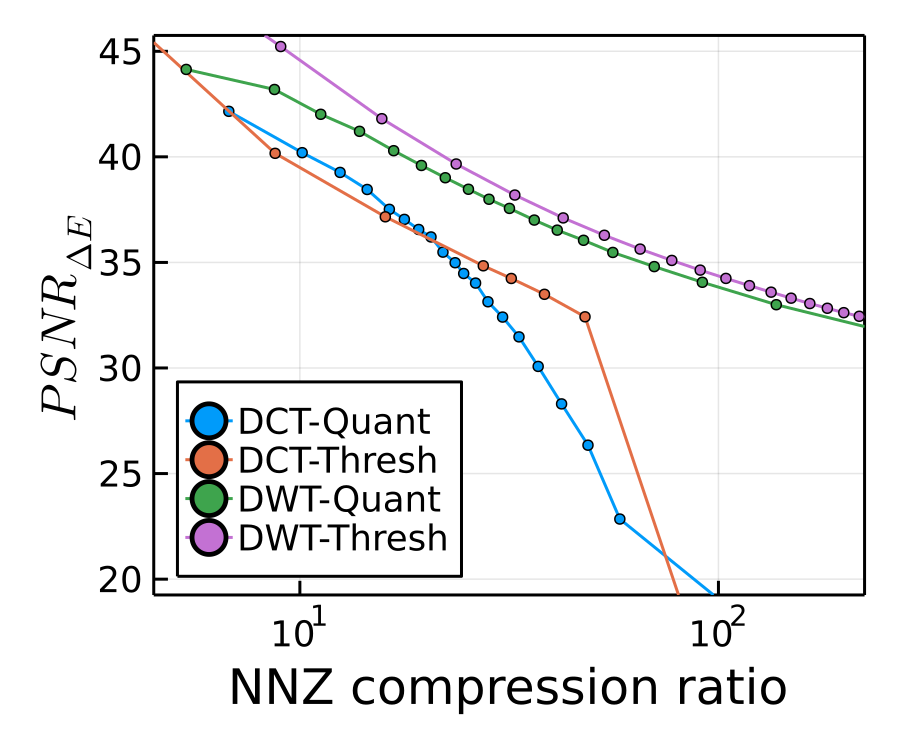
\includegraphics[width=0.48\columnwidth]{images/cr_psnr_plots/lighthouse/nnz_comparison.png}}
    \par
    \subfloat[monarch (RLE)]{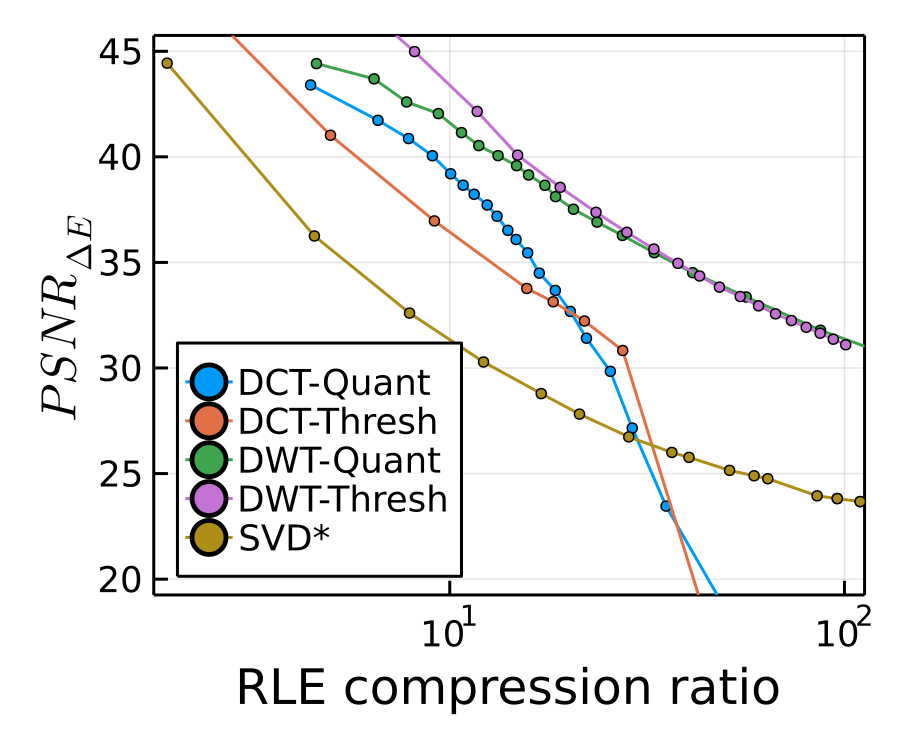
\includegraphics[width=0.48\columnwidth]{images/cr_psnr_plots/monarch_color/comparison.png}}
    \quad
    \subfloat[monarch (NNZ)]{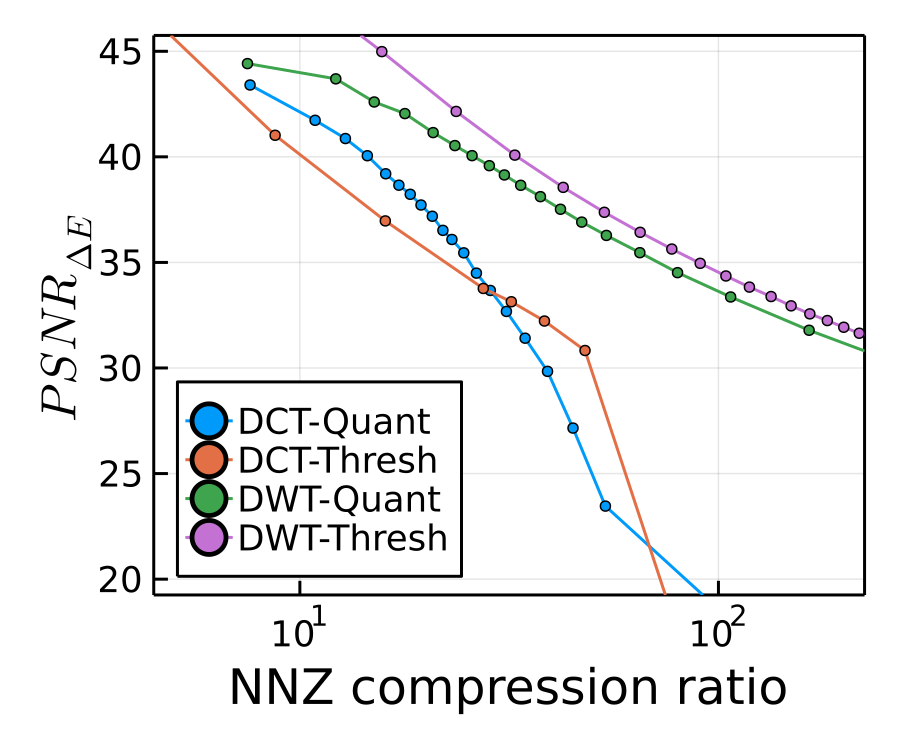
\includegraphics[width=0.48\columnwidth]{images/cr_psnr_plots/monarch_color/nnz_comparison.png}}
    \par
    \subfloat[airplane (RLE)]{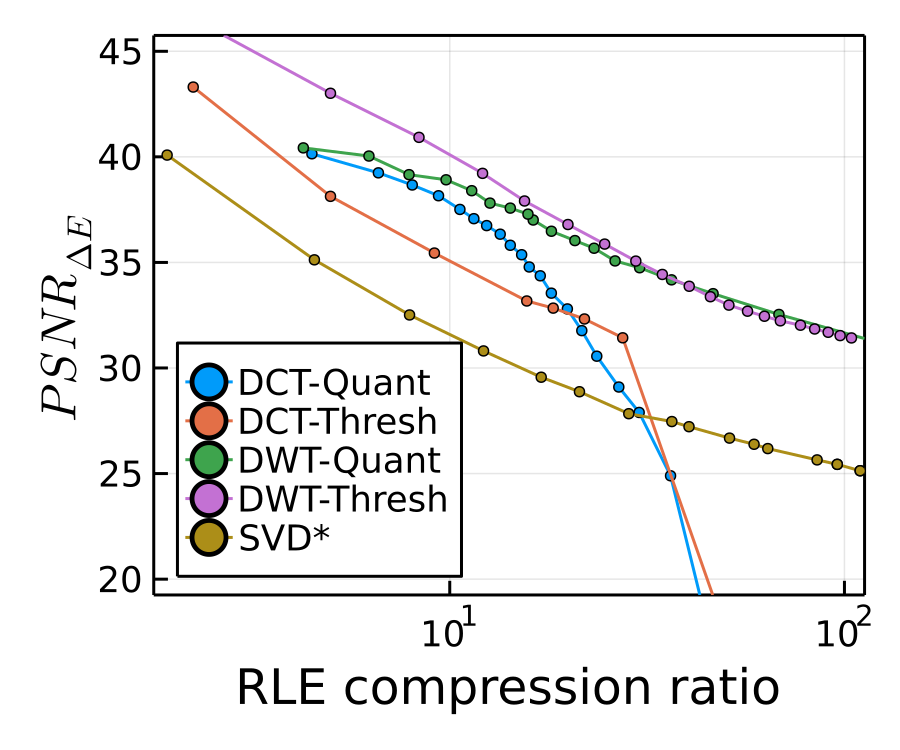
\includegraphics[width=0.48\columnwidth]{images/cr_psnr_plots/airplaneF16/comparison.png}}
    \quad
    \subfloat[airplane (NNZ)]{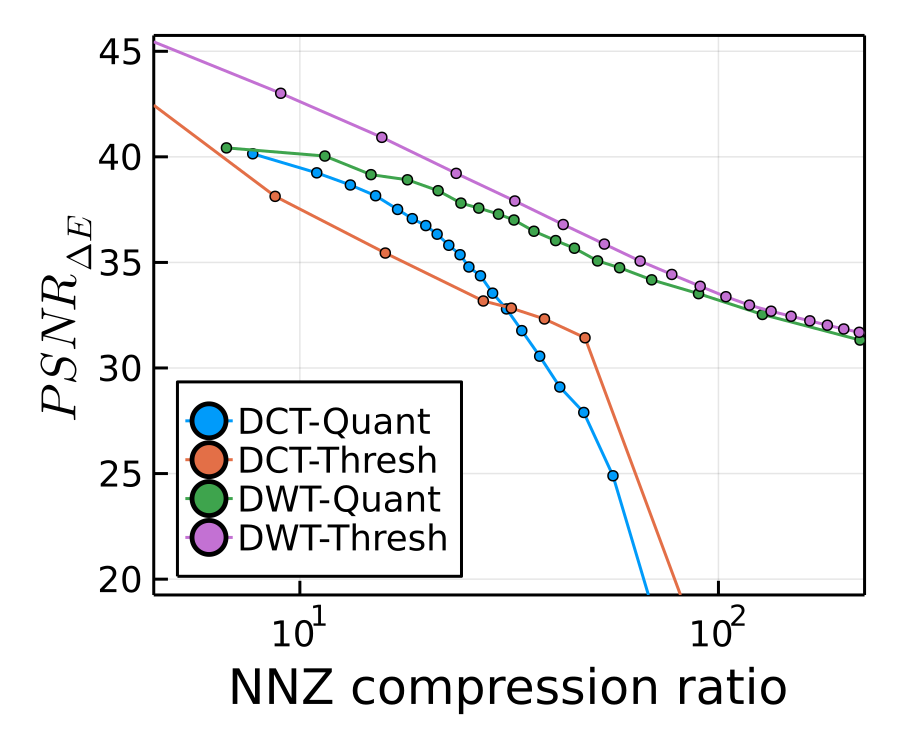
\includegraphics[width=0.48\columnwidth]{images/cr_psnr_plots/airplaneF16/nnz_comparison.png}}
    \caption{PSNR vs. compression ratio for various compression techniques on multiple images. Compression ratio is measured based on the number of bits required to store the run length encoding (RLE) and based on the ratio of nonzero values in the transform domain (NNZ). The SVD compression method uses a different compression scheme because it stores the compressed image in the singular value decomposition form. The fairest comparision for the SVD compression is to report its compression ratio along with the methods that use RLE.}
    \label{fig:cr_psnr_method_comparison}
\end{figure}

Figure \ref{fig:cr_psnr_method_comparison} is a comparison of the different compression techniques proposed in this work on the 5 test images.
The peak signal to noise ratio PSNR is plotted against the compression ratio for the various compression techniques.
Better compression schemes have a high PSNR for high compression ratios (i.e. towards the top right corner of the plot of PSNR vs. compression ratio)

\begin{figure*}
    \centering
    \subfloat[4:1 compression with tiled (tilesize = 8) DCT quantization. $PSNR_{\Delta E} = 31$dB]{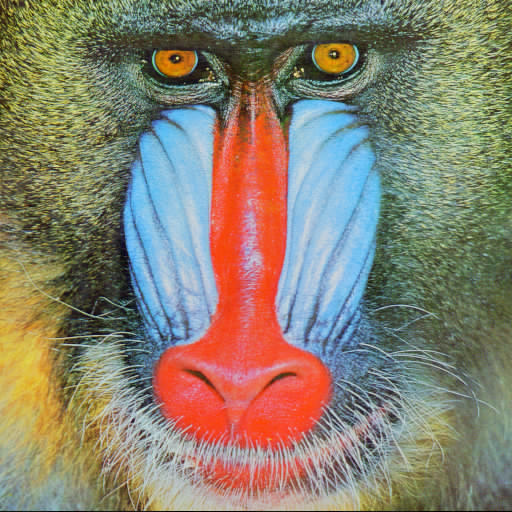
\includegraphics[width=0.3\textwidth]{images/mandrill_DCTQuant_4x_PSNR_31.png}}
    \quad
    \subfloat[32:1 compression with tiled (tilesize = 8) DCT quantization. $PSNR_{\Delta E} = 24$dB. Note the discoloration. Some of the individual $8\times8$ DCT basis vectors are visible in the furry areas of the mandrill.]{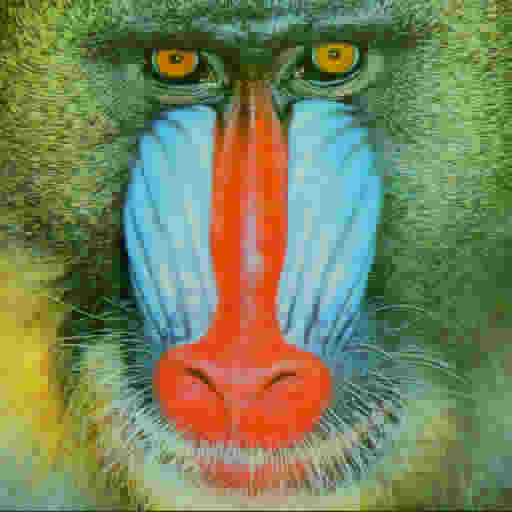
\includegraphics[width=0.3\textwidth]{images/mandrill_DCTQuant_32x_PSNR_24.png}}
    \quad
    \subfloat[45:1 compression with tiled (tilesize = 8) DCT quantization. $PSNR_{\Delta E} = 17$dB. This is the maximum compression level JPEG can offer for this image.]{
\includegraphics[width=0.3\textwidth]{images/mandrill_DCTQuant_45x_PSNR_17.png}}
    \par
    \subfloat[4:1 compression with tiled (tilesize = 16) DCT thresholding. $PSNR_{\Delta E} = 31$dB.]{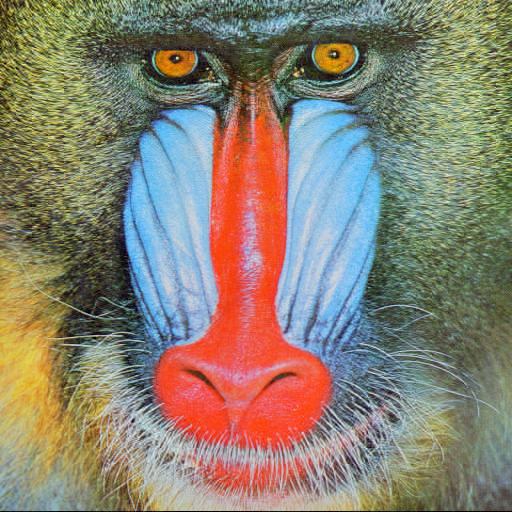
\includegraphics[width=0.3\textwidth]{images/mandrill_DCTThresh_4x_PSNR_31.png}}
    \quad
    \subfloat[32:1 compression with tiled (tilesize = 16) DCT thresholding. $PSNR_{\Delta E} = 27$dB. The tiling is noticeable now, especially around the red nose of the mandrill.]{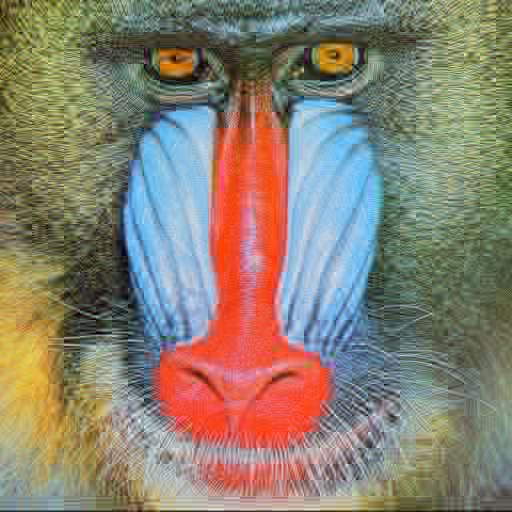
\includegraphics[width=0.3\textwidth]{images/mandrill_DCTThresh_32x_PSNR_27.png}}
    \quad
    \subfloat[96:1 compression with tiled (tilesize = 16) DCT thresholding. $PSNR_{\Delta E} = 26$dB. Most DCT coefficients have dropped, making individual DCT basis vectors visible in many of the tiles.]{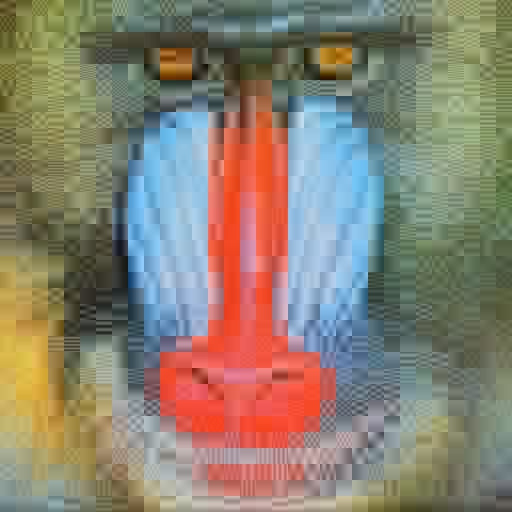
\includegraphics[width=0.3\textwidth]{images/mandrill_DCTThresh_96x_PSNR_26.png}}
    \par
    \subfloat[4:1 compression with non-tiled DCT thresholding. $PSNR_{\Delta E} = 30$dB.]{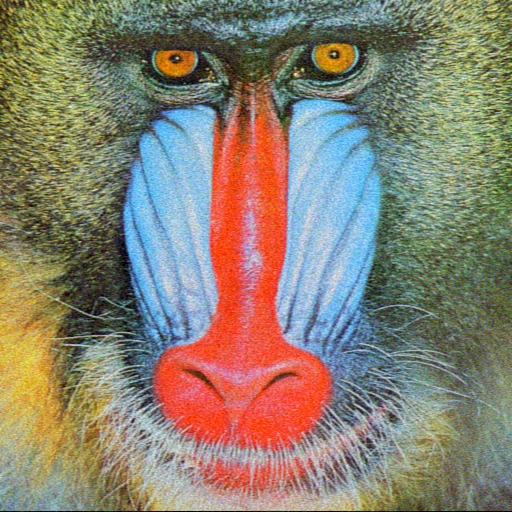
\includegraphics[width=0.3\textwidth]{images/mandrill_DCTThresh_4x_PSNR_30_largetile.png}}
    \quad
    \subfloat[32:1 compression with non-tiled DCT thresholding. $PSNR_{\Delta E} = 27$dB. Note the lack of high frequency clarity / sharpness.]{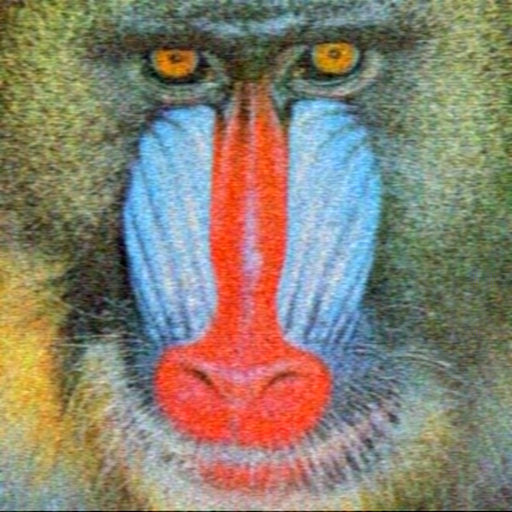
\includegraphics[width=0.3\textwidth]{images/mandrill_DCTThresh_32x_PSNR_27_largetile.png}}
    \quad
    \subfloat[97:1 compression with non-tiled DCT thresholding. $PSNR_{\Delta E} = 26$dB]{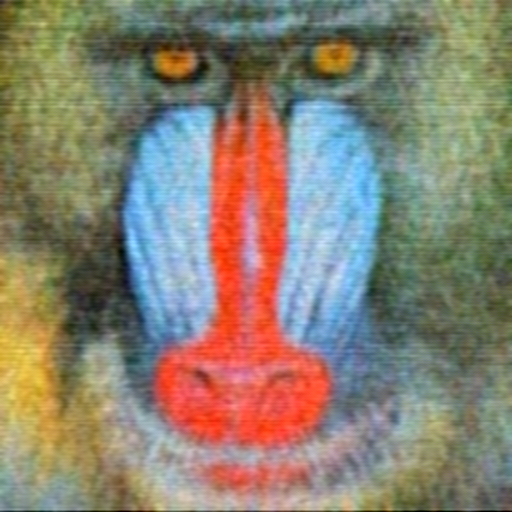
\includegraphics[width=0.3\textwidth]{images/mandrill_DCTThresh_97x_PSNR_26_largetile.png}}
    \caption{
        Typical compression artifacts of high compression ratios for DCT quantization and thresholding methods.
        Compression ratio is derived from the number of bits required to store the run length encoded quantized/thresholded transform of the image.
        Note the distortion caused by tiling and the fuzziness/striation caused by thresholding of the entire image.}
    \label{fig:dct_results}
\end{figure*}

Figure \ref{fig:dct_results} shows the compression artifacts that are common for DCT-based compression methods.
When performing tiling, it is common to observe individual DCT basis vectors filling individual tiles.
This occurs when the transform coefficients belonging to other basis vectors are set to zero by quantization or thresholding.

\begin{figure*}
    \centering
    \subfloat[4:1 compression with DWT quantization. $PSNR_{\Delta E} = 31$dB]{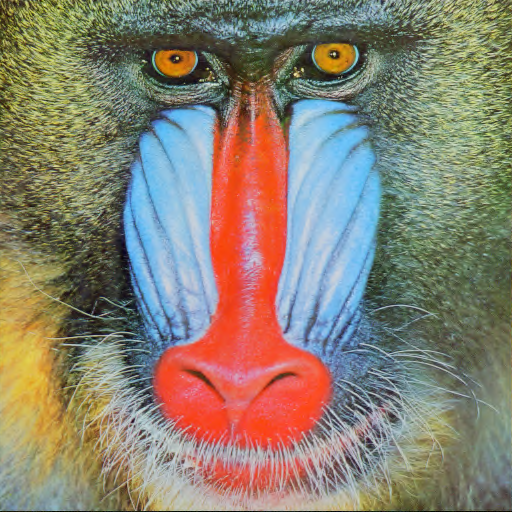
\includegraphics[width=0.3\textwidth]{images/mandrill_DWTQuant_4x_PSNR_31.png}}
    \quad
    \subfloat[32:1 compression with DWT quantization. $PSNR_{\Delta E} = 27$dB.]{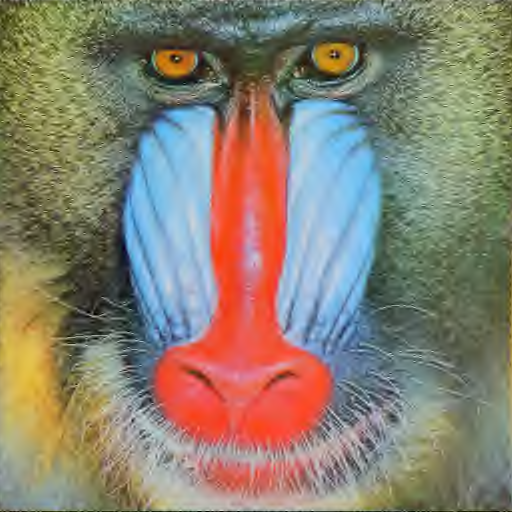
\includegraphics[width=0.3\textwidth]{images/mandrill_DWTQuant_32x_PSNR_27.png}}
    \quad
    \subfloat[93:1 compression with DWT quantization. $PSNR_{\Delta E} = 27$dB.]{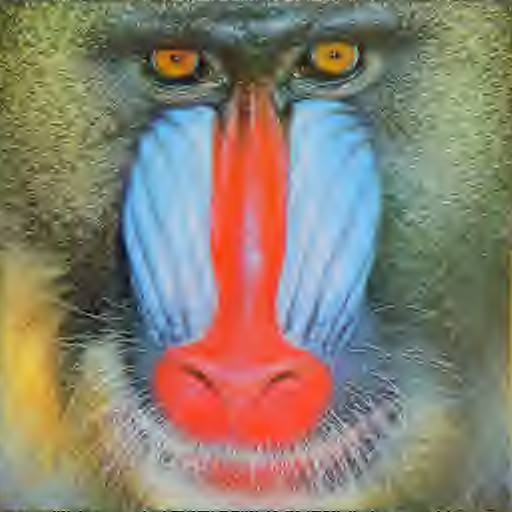
\includegraphics[width=0.3\textwidth]{images/mandrill_DWTQuant_93x_PSNR_27.png}}
    \par
    \subfloat[4:1 compression with DWT thresholding. $PSNR_{\Delta E} = 32$dB.]{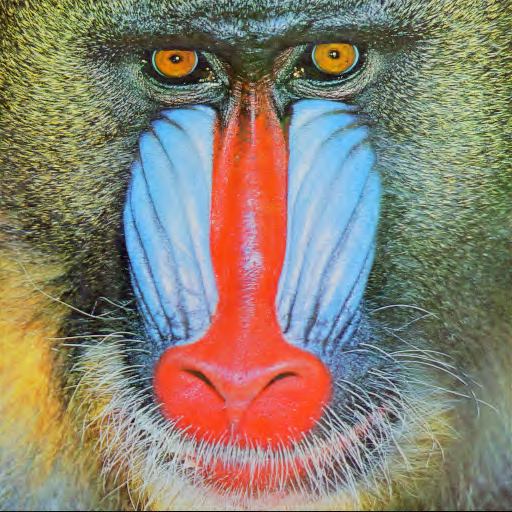
\includegraphics[width=0.3\textwidth]{images/mandrill_DWTThresh_4x_PSNR_32.png}}
    \quad
    \subfloat[32:1 compression with DWT thresholding. $PSNR_{\Delta E} = 27$dB.]{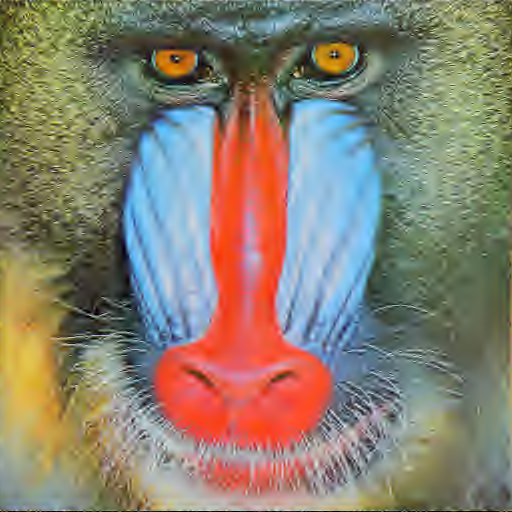
\includegraphics[width=0.3\textwidth]{images/mandrill_DWTThresh_32x_PSNR_27.png}}
    \quad
    \subfloat[93:1 compression with DWT thresholding. $PSNR_{\Delta E} = 27$dB.]{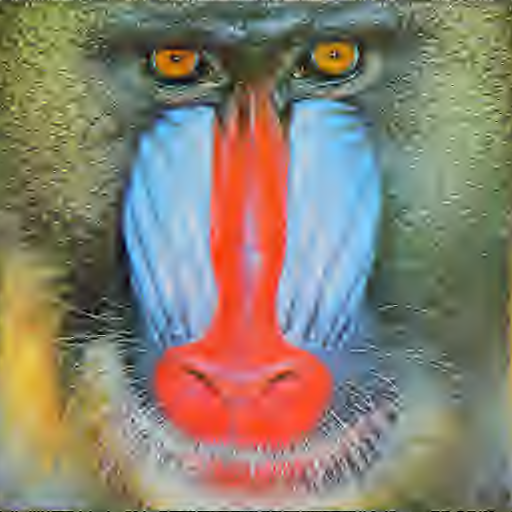
\includegraphics[width=0.3\textwidth]{images/mandrill_DWTThresh_93x_PSNR_27.png}}
    \caption{
        Compression artifacts from DWT thresholding and quantization.
        The blurriness with a few dots of sharpness here and there (most noticeable in highly compressed images) is one of the hallmarks of wavelet-based compression schemes.
        This phenomenon occurs because the high frequency wavelets are also highly localized in space, so the largest high frequency wavelet coefficients which aren't truncated or quantized create this speckling pattern.}
    \label{fig:dwt_results}
\end{figure*}

\begin{figure*}
    \subfloat[4:1 compression with SVD. $PSNR_{\Delta E} = 29$dB]{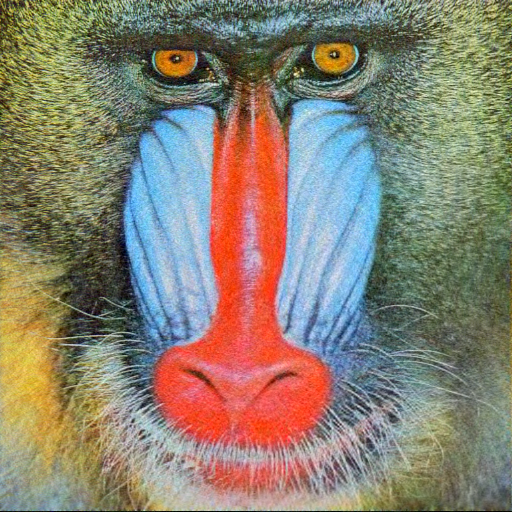
\includegraphics[width=0.3\textwidth]{images/mandrill_SVD_4x_PSNR_29.png}}
    \quad
    \subfloat[32:1 compression with SVD. $PSNR_{\Delta E} = 25$dB.]{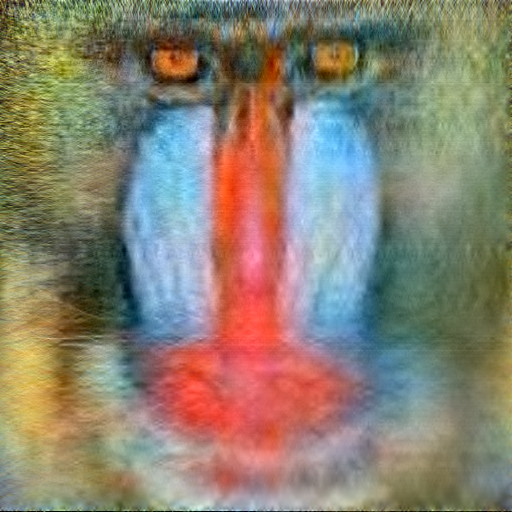
\includegraphics[width=0.3\textwidth]{images/mandrill_SVD_32x_PSNR_25.png}}
    \quad
    \subfloat[110:1 compression with SVD. $PSNR_{\Delta E} = 23$dB.]{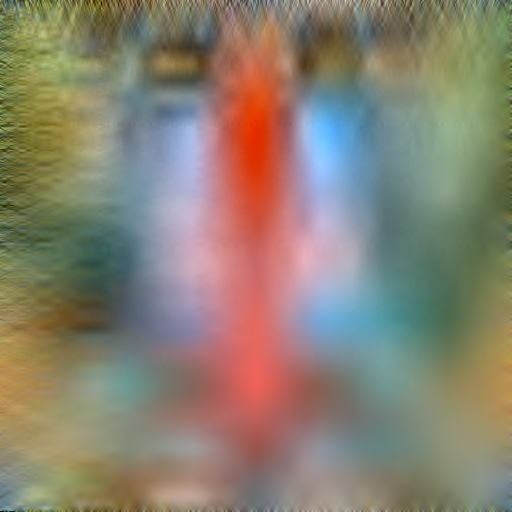
\includegraphics[width=0.3\textwidth]{images/mandrill_SVD_110x_PSNR_23.png}}
    \caption{Compression artifacts from SVD rank reduction.}
    \label{fig:svd_results}
\end{figure*}

Figure \ref{fig:dwt_results} shows the results of applying quantization and thresholding to the DWT of an image.
High levels of compression cause the image to appear blurry with a few specks of sharpness scattered around the image.
This is caused by the high spatial locality of high frequency wavelet basis vectors.
Since most of the high frequency wavelet coefficients are small, they are set to zero by thresholding or quantization.
This causes the blurring effect, since the effect is similar to applying a lowpass filter or gaussian blur to an image.
The few nonzero wavelet coefficients from the high frequency subbands that aren't set to zero cause the small specks of sharpness.

Figure \ref{fig:svd_results} shows the results for varying levels of compression with the SVD method.
The SVD-based compression method appears to perform pretty poorly in comparison to thresholding and quantization of the image DWT.

\section{Discussion}

\subsection{Poor performance of SVD compression}

As seen in Figures \ref{fig:cr_psnr_method_comparison} and \ref{fig:dwt_results}, the SVD rank-reduction compression method produces very poor results compared to the other methods.
Initially, it might seem useful to use the SVD of the wavelet transform of the image, since intuitively, the wavelet transform of the image separates the image into various components with different relevance, and so it might be easier to compress the image without substantially altering the perceived image quality.
However, since the wavelet transform is a linear operation (see Equation \ref{eqn:2Dtransform}), it's SVD is identical, apart from a basis transformation of the singular vector matrices:

\begin{IEEEeqnarray}{rCl}
    \mathbf{X} & = & \mathbf{U}\mathbf{\Sigma}\mathbf{V}^T \\
    \mathbf{\widetilde{X}} & = & \mathbf{\Phi}\mathbf{X}\mathbf{\Phi}^T \\
    & = & \mathbf{\Phi}\mathbf{U}\mathbf{\Sigma}\mathbf{V}^T\mathbf{\Phi}^T \\
    & = & \left(\mathbf{\Phi}\mathbf{U}\right)\mathbf{\Sigma}\left(\mathbf{\Phi}\mathbf{V}\right)^T \\
    \mathbf{\widetilde{X}} & = & \mathbf{U}_{\Phi}\mathbf{\Sigma}\mathbf{V}_{\Phi}^T
    \label{eqn:svd_dwt_linear_relation}
\end{IEEEeqnarray}

Based on this equation, there is no advantage to be gained by taking the SVD of the transform of the image.
Thus, there is no way for the SVD to take advantage of the wavelet transform's ability to separate perceptually relevant features of an image \cite{hvsWavelet}.
Therefore, it is somewhat unsurprising that the SVD rank-reduction method is outperformed by compression methods such as quantization and thresholding that operate on of the DWT of an image.

\subsection{DCT vs. DWT}
As can be seen in comparing Figure \ref{fig:dct_results} with \ref{fig:dwt_results}, the compression methods which use the wavelet transform are capable of maintaining the key qualities of the original image while achieving much higher compression ratios.
This effect can be seen quantitatively in the comparison of PSNR to compression ratio for DCT and DWT-based methods in Figure \ref{fig:cr_psnr_method_comparison}.
Again, this behavior is explained by the wavelet transform's ability to pick out perceptually relevant details from an image \cite{hvsWavelet}.
Another key advantage of the wavelet transform is the spatial locality of its basis vectors,
which enables more accurate reconstruction of compression applied to tiled images (not shown here),
since the wavelet coefficients capture spatial information about the different frequencies present in a tile and can place sharp features in the correct place,
somewhat reducing the perceived ``blockiness" effect that is characteristic of compression algorithms which use tiling.

\subsection{Thresholding vs. Quantization}
Even though thresholding can often produce better PSNR than quantization for moderate amounts of compression (see Figure \ref{fig:cr_psnr_method_comparison}), the end user of a lossy image compression algorithm is likely to care primarly about the final image quality, rather than the final file size.
Thresholding makes it very easy to control the number of bits required to store the final image, however it doesn't account for differences in how easy it is to compress an image.
As can be seen in Figure \ref{fig:cr_psnr_method_comparison}, the monarch is much easier to compress (higher PSNR for the same compression ratio) than the mandrill due to the fact that it's a less ``busy" image, so more of the wavelet coefficients are small and setting them to zero or reducing the effective number of bits used to represent them is less perceptible.
For example, thresholding the smallest 60\% of the wavelet coefficients will have a very different impact on the compressed PSNR of the two images,
whereas applying quantization with the same quality factor for the two images will result in similar compressed image qualities.
It's possible that using the entropy of the different subbands of the wavelet transform as a metric for image complexity could work as a method for estimating the required threshold ratio to achieve a certain final image quality, however this idea was not explored in this work.

\begin{thebibliography}{00}
    \bibitem{imgProcessingTinkuAcharya} T. Acharya and A. K. Ray, ``Image Processing: Principles and Applications" 1st ed. \textit{Wiley}, pp 329 (2005)
    \bibitem{scnn} A. Parashar, et. al., ``SCNN: An Acclerator for Compressed-sparse Convolutional Neural Networks", \textit{Proceedings of ISCA '17}, pp. 27-40 (2017)
    \bibitem{hvsWavelet} T. P. O'Rourke and R. L. Stevenson,``Human Visual System Based Wavelet Decomposition for Image Compression,'' \textit{Journ. Visual Comm. and Image Representation}, vol. 6, pp. 109-121, (1955)
    \bibitem{jpegStd} G. Hudson, A. L{\'e}ger, B. Niss, I. Sebesty{\'e}n, J. Vaaben, ``JPEG-1 standard 25 years: past, present, and future reasons for a success,", \textit{Journ. Electronic Imaging}, vol. 27, (2018).
    \bibitem{strang} G. Strang, ``Linear Algebra and Learning from Data", pp. 72-74 (2019).
\end{thebibliography}

\end{document}
